\section{Experimental Methodology}
\label{sec:method}

To evaluate the effectiveness of TeraHeap, we conduct a
set of experiments using various workloads from the Spark Bench suite
and graphalytics library for Giraph
on a real-world cluster. Our experimental methodology consists of
several steps. First, we install and configure Spark, Giraph and OpenJDK8 on the
cluster. We use Spark's-Giraph's default configuration settings for our
experiments, except for the garbage collector settings, which we tune
according to the requirements for TeraHeap.

We select four workloads from the Spark Bench suite that represent
different types of data processing, such as machine learning and graph
processing, (and SQL queries ???). We run each workload using TeraHeap
and compare it with the performance of the same
workload using the default configuration, garbage collector tuning,
and heap offloading approaches.

When running multiple colocated instances of a frameowork,
we utilize all the available DRAM provided by our server leaving 8-10
GB for the Operating System, while increasing the number of
instances that are executed. We show that by using TeraHeap, each
individual instance requires less memory therefore memory becomes
available for more instances to be deployed, achieving more total
throughput than Native Spark-Giraph in similar time windows.

To measure the performance of TeraHeap, we use several metrics,
including server throughput, memory usage, and execution time. We
measure server throughput as the megabytes of the dataset processed
per second, memory usage as the amount of memory used during data
processing, and execution time as the time taken to complete the
workload.

We repeat each experiment several times to ensure statistical
significance and calculate the mean and standard deviation of the
metrics for each approach.

In summary, our experimental methodology involves setting up a
real-world cluster, selecting appropriate workloads, measuring
performance using several metrics, and repeating each experiment
several times to ensure statistical significance. By following this
methodology, we can evaluate the effectiveness of TeraHeap
for improving server throughput for managed big data
analytics.

\begin{table}[t!]
  \centering
  \caption{Server Specifications}
  \label{tab:server-specs}
  \begin{tabular}{|c|c|}
    \hline
    \textbf{Component} & \textbf{Specification} \\
    \hline
    Memory & 8x DDR4 32-GB \\
    CPU & 2x Intel Xeon E5-2630 2.4 GHz \\
    Cores per CPU & 16 \\
    NUMA Islands & 2 \\
    Cores per NUMA island & 16 \\
    L1 Cache & 512 KB \\
    L2 Cache & 2 MB \\
    L3 (LLC) Cache & 20 MB \\
    Storage & 2x 1.8 TB KVS NVMe \\
    \hline
  \end{tabular}
\end{table}

\subsection{Server Characteristics}
The server used in our experiments is a high-performance machine with
hardware specifications found in real-world clusters.
It is equipped with 8x DDR4 32-GB 2.4 GHz 64-bit DIMMs, providing a
total of 256 GB of memory. The DDR4 memory technology is known for its
high bandwidth and low power consumption, making it ideal for
data-intensive applications like big data analytics. The server also
features 2x Intel Xeon E5-2630 2.4 GHz 16-core 64-bit CPUs, split into 2
NUMA islands. Each core has 512 KB L1, 2 MB L2, and 20 MB L3 (LLC) cache.
The Xeon E5-2630 CPU is a high-performance processor designed for data
centers, offering a high core count, high clock speed, and advanced
features like hyper-threading and Turbo Boost. The large L3 cache
helps reduce memory latency, enabling faster data access for CPU-bound
workloads. In addition to the powerful CPUs and memory, the server
also has 2x KVS NVMe storage devices. NVMe is a high-performance
storage technology that uses PCIe to connect directly to the CPU,
providing low latency and high throughput. The KVS (Key-Value Store)
storage devices are designed for fast, random access to data, making
them ideal for storing and retrieving large amounts of data in big
data applications. Overall, the server's hardware specifications make
it a powerful platform for conducting experiments on managed big data
analytics and evaluating the performance of TeraHeap. 

\subsection{Native Spark Configuration}
We use Spark v3.3.0 with Kryo Serializer, a state-of-the-art highly
optimized S/D Library for Java that Spark recommends. We run Spark
with Native OpenJDK8 as a baseline. We use the Parallel Scavenge
garbage collector which is the one TeraHeap is implemented for.
Parallel Scavenge is also the go-to collector for applications that
need high throughput like Spark. We use an executor with eight mutator
threads for each instance of Spark we deploy on our server. For
Parallel Scavenge, we use 8 GC Threads for minor GC and the default
single-threaded old generation GC. Spark uses the MEMORY-AND-DISK
storage level to place executor memory (heap) in DRAM and cache RDDs
in the on-heap cache, up to 50\% of the total heap size. Any remaining
RDDs are serialized in the off-heap cache over an NVMe SSD. This
device is also used by Spark for shuffling. We run each instance of
Spark in a cgroup containing two JVM instances, one for Spark driver
and one for Spark executor and all the processes needed to measure
performance for this instance. Each cgroup has a limited DRAM Budget.
A part of the budget is the capacity of the Java Heap which, for the
rest of the paper, we call H1. We do this in order to be sure that
every instance of Spark running on our server has a fair amount of
DRAM available for it to use. We choose to try two different amounts
for H1, 40\% and 80\% of total DRAM budget. 80\% is the go-to
percentage of total DRAM RedHat uses in its datacenters [?]. What
remains is used by JVM for Native memory (i.e. CodeCache) and for the
operating system's Page Cache. In order to avoid inter-NUMA island
interference, we shut down the 16 cores belonging to the second island
thus leaving 16 active cores. We also turn off the swapper, because it
adds significant overhead and makes it difficult to understand the
results of the experiments conducted.

\subsection{Native Giraph Configuration}
Empty

\subsection{TeraHeap}
\subsubsection{What is TeraHeap?}
TeraHeap is a high-capacity managed heap that is memory-mapped over a
fast storage device (preferrably block-addresable NVMe or
byte-addresable NVM). The high speeds these kind of devices operate
in, erase any overhead caused by the use of MMIO. TeraHeap is designed
as an extension of the main Java Heap. It holds specific long-lived
objects that have the same lifetime span. This enables TeraHeap to
operate as a GC-free heap that can delete entire regions of objects at
once without the need to scan the heap over and over again for dead
objects. This would be a performance kill as it would require scans
over the storage device. The two main contributions of TeraHeap are
the following: 1) MMIO keeps the objects that reside in the storage
device deserialized, thus eliminating the need for
Serialization/Deserialization 2) As discussed, TeraHeap reduces GC overheads
without wasting DRAM by avoiding scans on long-lived objects.

\subsubsection{Spark Configuration}
The configuration for TeraHeap is pretty much the same as for Native
Spark, with some necessary differences to achieve our goal. TeraHeap
is mapped to a different storage device (NVMe) than that Spark is
using for shuffling. We do this in order for TeraHeap to utilize its
device to its fullest. MMIO allows TeraHeap Spark to run in
MEMORY-ONLY storage level as Spark remains unaware of using any device and
the OS takes control of the I/O. We also make the same decisions for
the DRAM budget trying different amounts for H1, 40\% and 80\% of
total DRAM budget. By doing that, we have different configurations
where H1 dominates PageCache and the reverse showing what the needs of
different Spark applications are. 

\subsubsection{Giraph Configuration}
Empty

\subsection{What workloads did we choose to use for our experiments and why?}
For our experiments, we selected four specific workloads from two
different categories of the Spark Bench suite: Page Rank and Connected
Component from GraphX and Linear Regression and Logistic Regression
from MLLib. The primary reason for selecting these workloads is that
they represent different types of big data analytics tasks: PageRank
and Connected Component are graph-based workloads, while
LinearRegression and LogisticRegression are machine learning
workloads. By selecting workloads from both categories, we can
investigate the performance of TeraHeap across a range of
big data analytics tasks. Furthermore, all of them are
well-established workloads that are commonly used for benchmarking big
data analytics systems, making them a suitable choice for our
experiments. Overall, the selection of these workloads allows us to
evaluate the performance of TeraHeap in a variety of contexts and
provide insights into the effectiveness of TeraHeap for improving
server throughput in managed big data analytics systems.

\subsubsection{PageRank}
PageRank is a widely used graph-based algorithm that measures the
importance of nodes in a network. It has become a popular benchmark
for evaluating the performance of distributed systems, including big
data analytics systems like Apache Spark. PageRank is computationally
intensive and requires significant memory and I/O resources, making it
a suitable workload for evaluating the performance of our TeraHeap
for improving server throughput. Additionally, PageRank is a
common algorithm in real-world applications, such as search engines
and social networks, making it relevant for practical use cases.

\subsubsection{LinearRegression}
LinearRegression is a machine learning algorithm that is used to
predict numerical values based on input data. It is a well-known and
widely used algorithm in machine learning, and is commonly used for
regression analysis in fields such as economics, finance, and
engineering. LinearRegression is computationally intensive and
requires significant memory and I/O resources, making it a suitable
workload for evaluating the performance of TeraHeap for
improving server throughput. Furthermore, the inclusion of a machine
learning workload like LinearRegression allows us to investigate the
performance of TeraHeap across different types of big data
analytics tasks and gain insights into the effectiveness of TeraHeap
for improving server throughput in a range of contexts.

\subsubsection{Logistic Regression}
LogisticRegression is a machine learning algorithm that is used to
model the probability of a binary or categorical outcome based on one
or more independent variables. It is commonly used in predictive
analytics to classify data based on historical data. In Spark-bench,
LogisticRegression is implemented as a machine learning workload,
where the dataset is represented as an RDD of feature vectors and
labels. The LogisticRegression workload involves training a logistic
regression model on the dataset, using an iterative optimization
algorithm such as gradient descent. The workload is computationally
intensive and requires a significant amount of memory to store the
dataset and model parameters.

\subsubsection{Connected Component}
ConnectedComponent is a graph algorithm that is used to identify the
connected components of a graph. It is commonly used in social network
analysis to identify clusters of users with similar interests or
relationships. In Spark-bench, ConnectedComponent is implemented as a
graph processing workload, where the graph is represented as an RDD of
edges and vertices. The ConnectedComponent workload involves iterating
over the graph, identifying the connected components of each node, and
merging the components as necessary. The workload is computationally
intensive and requires a significant amount of memory to store the
graph.


\begin{figure*}[ht!]
    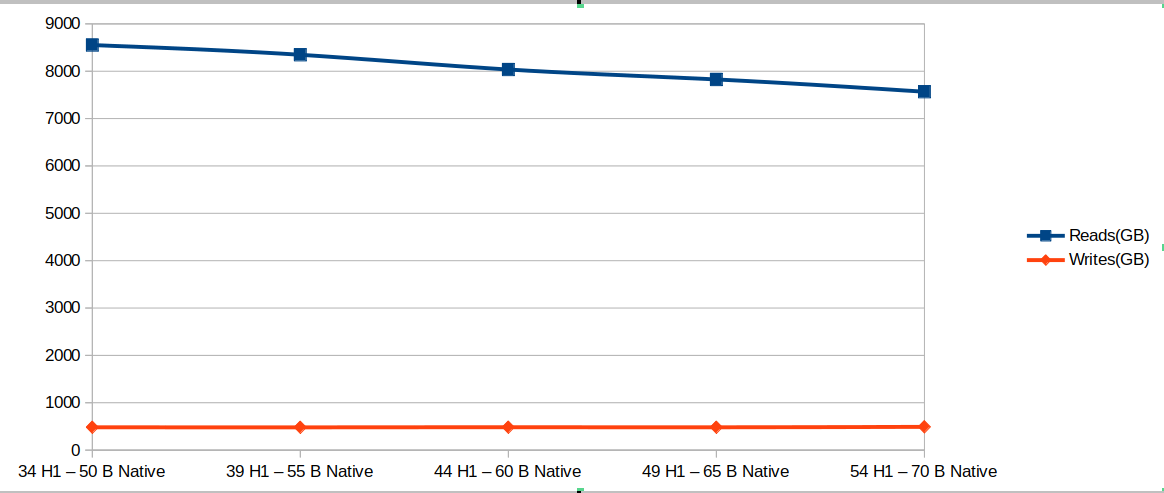
\includegraphics[width=12cm,height=6cm]{./fig/gcs_linr_h1_native.png}
    \caption{Number of GCs over time for H1 Linear Regression Native
    Spark investigation.}
    \label{fig:gcs_linr_h1_native}
\end{figure*}

\begin{figure*}[ht!]
    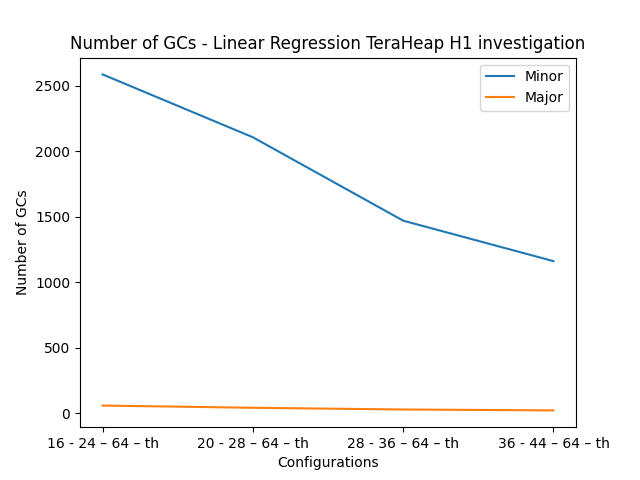
\includegraphics[width=12cm,height=6cm]{./fig/gcs_linr_h1_th.png}
    \caption{Number of GCs over time for H1 Linear Regression TeraHeap
    Spark investigation.}
    \label{fig:gcs_linr_h1_th}
\end{figure*}

\begin{figure*}[ht!]
    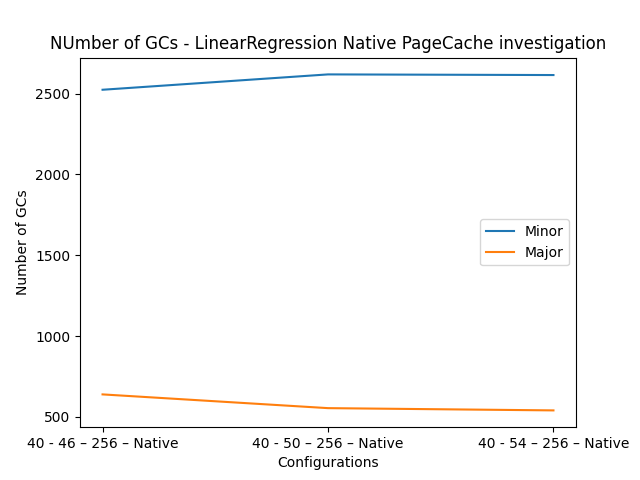
\includegraphics[width=12cm,height=6cm]{./fig/gcs_linr_pc_native.png}
    \caption{Number of GCs over time for Page Cache Linear Regression
    Native Spark investigation.}
    \label{fig:gcs_linr_pc_native}
\end{figure*}

\begin{figure*}[ht!]
    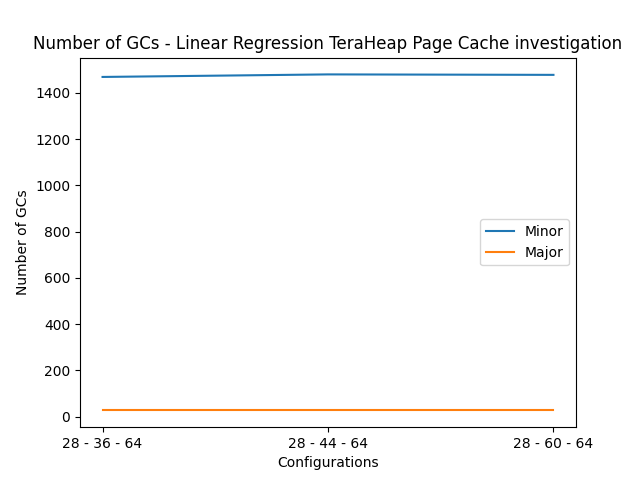
\includegraphics[width=12cm,height=6cm]{./fig/gcs_linr_pc_th.png}
    \caption{Number of GCs over time for Page Cache Linear Regression
    TeraHeap Spark investigation.}
    \label{fig:gcs_linr_pc_th}
\end{figure*}
\iffalse
\begin{figure*}[ht!]
    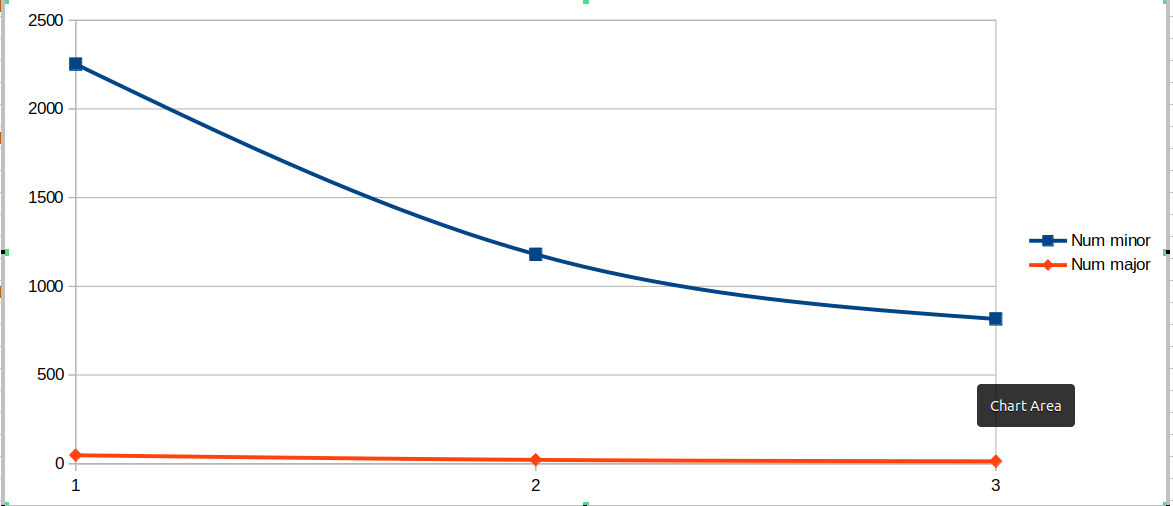
\includegraphics[width=12cm,height=6cm]{./fig/gcs_pr_h1_th.png}
    \caption{Number of GCs over time for H1 Page Rank TeraHeap Spark
    investigation.}
    \label{fig:gcs_pr_h1_th}
\end{figure*}
\fi
\begin{figure*}[ht!]
    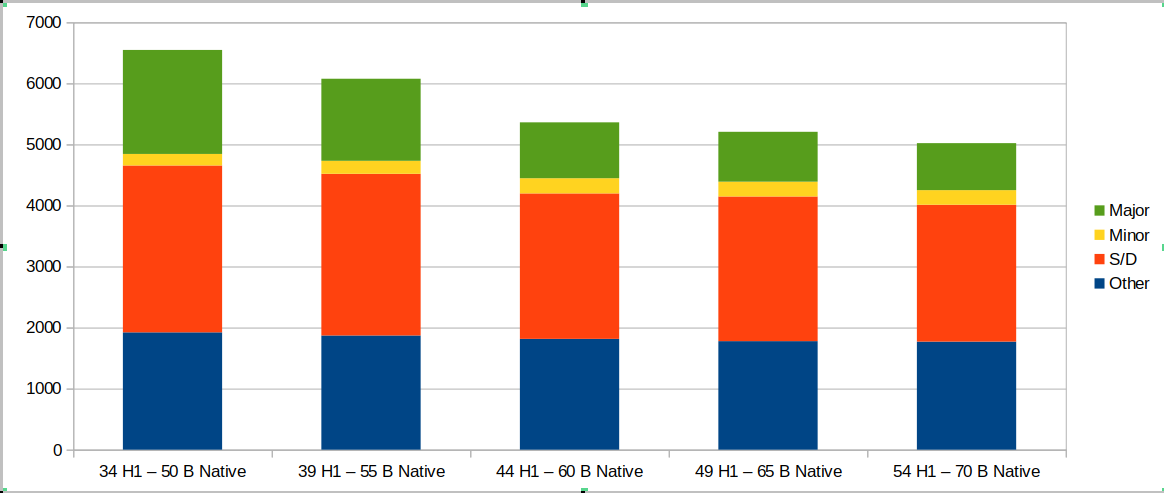
\includegraphics[width=12cm,height=6cm]{./fig/linr_h1_native.png}
    \caption{Execution time breakdown for H1 Linear Regression Native
    Spark investigation.}
    \label{fig:linr_h1_native}
\end{figure*}

\begin{figure*}[ht!]
    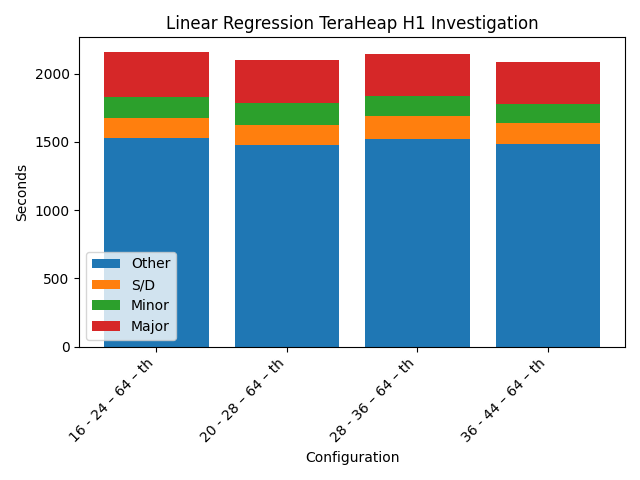
\includegraphics[width=12cm,height=6cm]{./fig/linr_h1_th.png}
    \caption{Execution time breakdown for H1 Linear Regression
    TeraHeap Spark investigation.}
    \label{fig:linr_h1_th}
\end{figure*}

\begin{figure*}[ht!]
    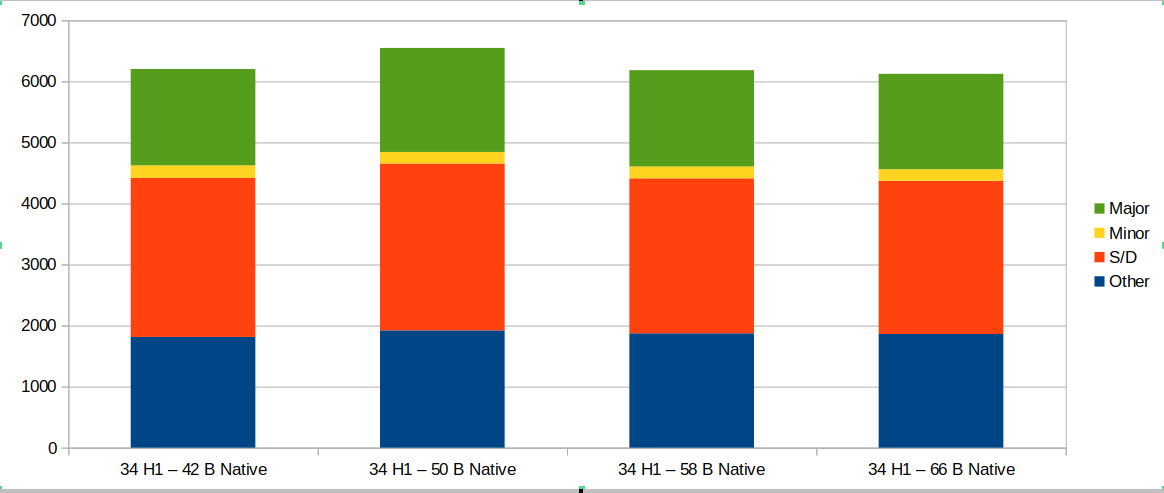
\includegraphics[width=12cm,height=6cm]{./fig/linr_pc_native.png}
    \caption{Execution time breakdown for Page Cache Linear Regression
    Native Spark investigation.}
    \label{fig:linr_pc_native}
\end{figure*}

\begin{figure*}[ht!]
    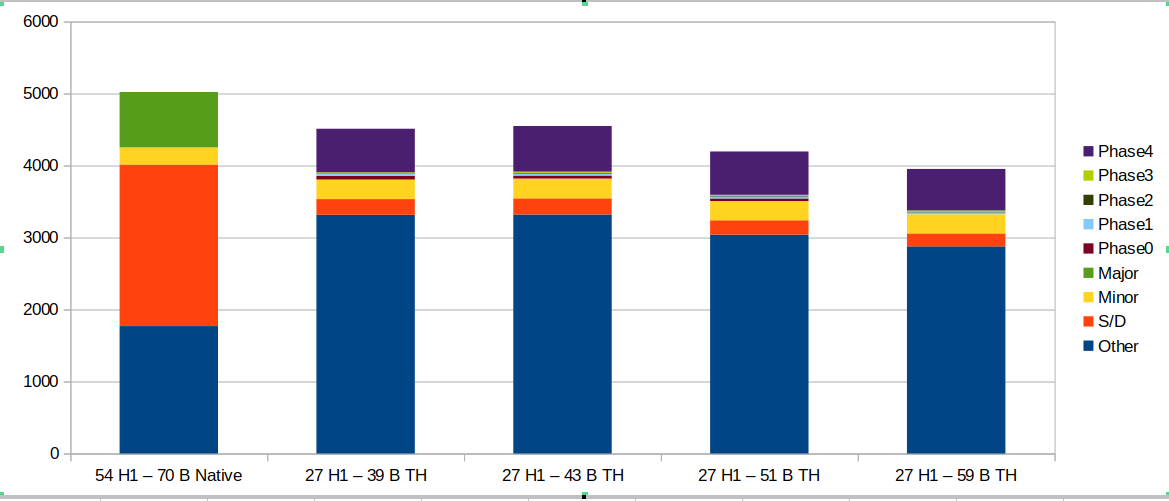
\includegraphics[width=12cm,height=6cm]{./fig/linr_pc_th.png}
    \caption{Execution time breakdown for Page Cache Linear Regression TeraHeap Spark investigation.}
    \label{fig:linr_pc_th}
\end{figure*}

\begin{figure*}[ht!]
    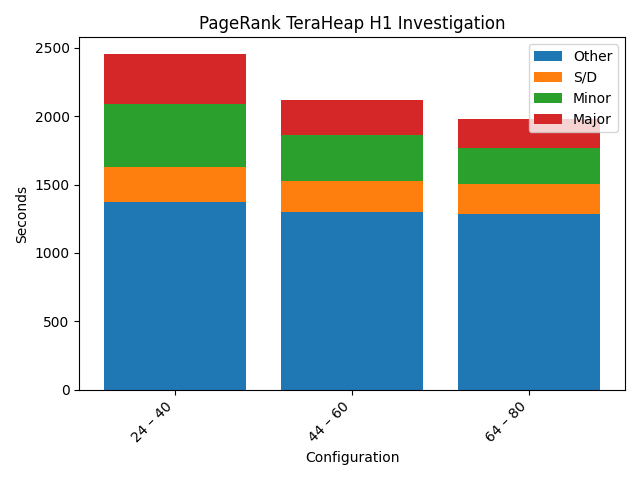
\includegraphics[width=12cm,height=6cm]{./fig/pr_h1_th.png}
    \caption{Execution time breakdown for H1 Page Rank TeraHeap Spark
    investigation.} 
    \label{fig:pr_h1_th}
\end{figure*}

\begin{figure*}[ht!]
    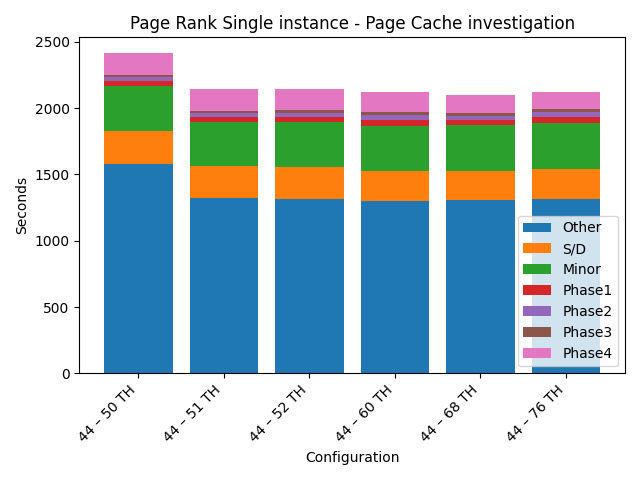
\includegraphics[width=12cm,height=6cm]{./fig/pr_pc_th.png}
    \caption{Execution time breakdown for PageCache Page Rank TeraHeap
    Spark investigation.}
    \label{fig:pr_pc_th}
\end{figure*}

\begin{figure*}[ht!]
    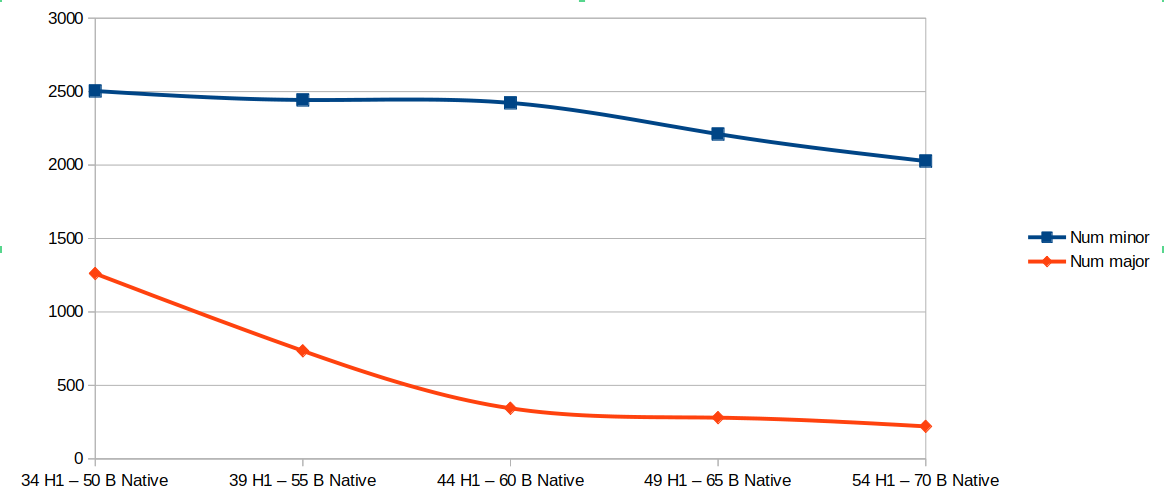
\includegraphics[width=12cm,height=6cm]{./fig/rw_linr_h1_native.png}
    \caption{Read-Write traffic over time for H1 Linear Regression
    Native Spark investigation.}
    \label{fig:rw_linr_h1_native}
\end{figure*}

\begin{figure*}[ht!]
    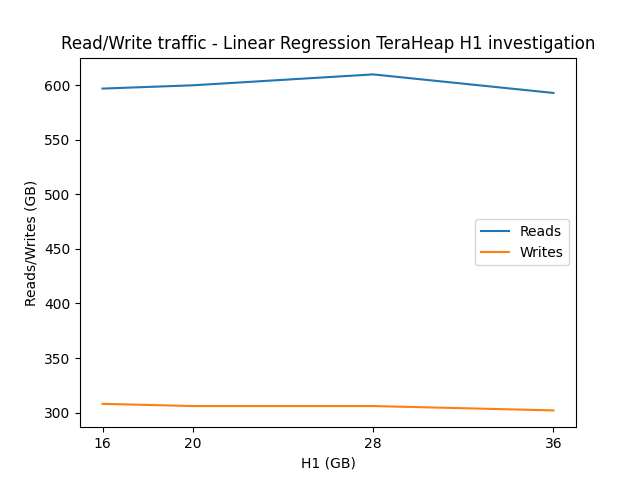
\includegraphics[width=12cm,height=6cm]{./fig/rw_linr_h1_th.png}
    \caption{Read-Write traffic over time for H1 Linear Regression
    TeraHeap Spark investigation.}
    \label{fig:rw_linr_h1_th}
\end{figure*}

\begin{figure*}[ht!]
    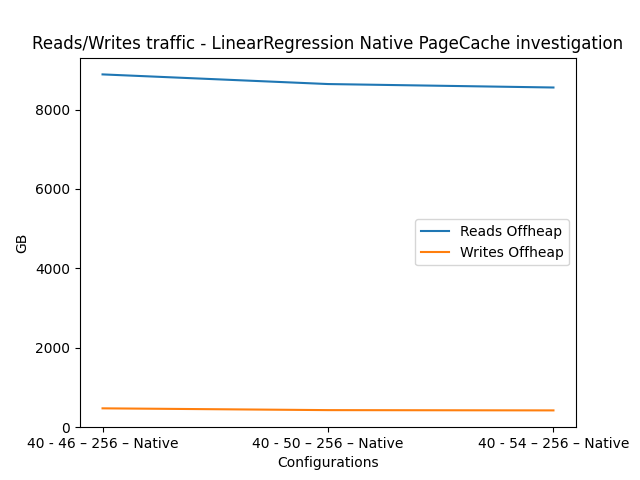
\includegraphics[width=12cm,height=6cm]{./fig/rw_linr_pc_native.png}
    \caption{Read-Write traffic over time for PageCache Linear
    Regression Native Spark investigation.}
    \label{fig:rw_linr_pc_native}
\end{figure*}

\begin{figure*}[ht!]
    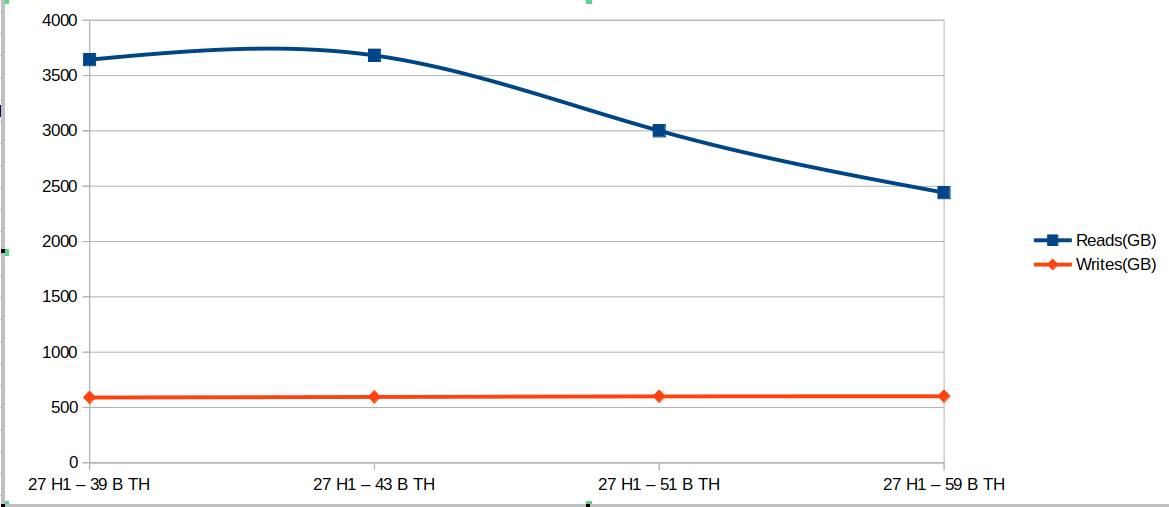
\includegraphics[width=12cm,height=6cm]{./fig/rw_linr_pc_th.png}
    \caption{Read-Write traffic over time for PageCache Linear
    Regression TeraHeap Spark investigation.}
    \label{fig:rw_linr_pc_th}
\end{figure*}

\begin{figure*}[ht!]
    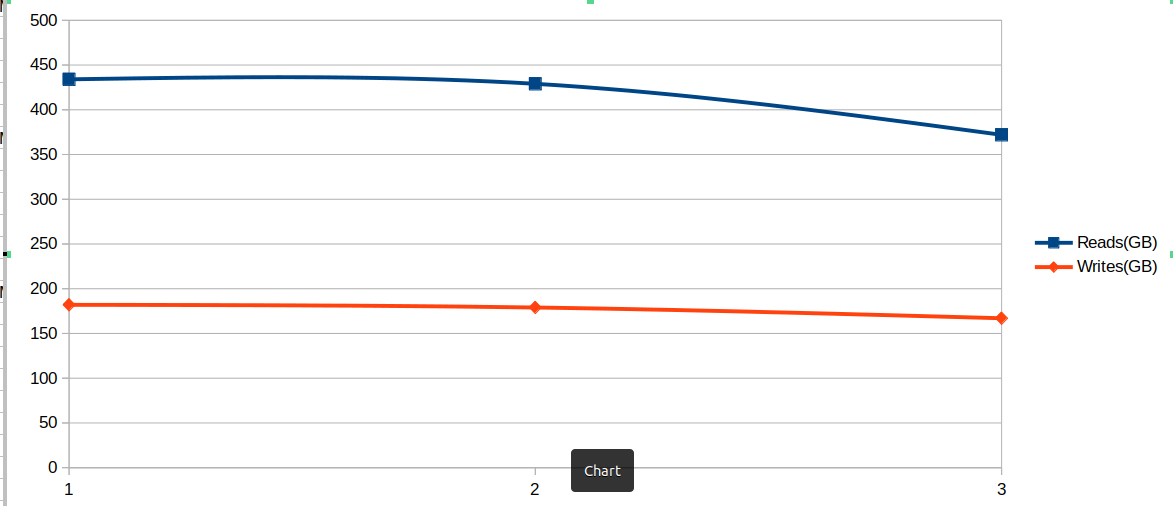
\includegraphics[width=12cm,height=6cm]{./fig/rw_pr_h1_th.png}
    \caption{Read-Write traffic over time for H1 Page Rank TeraHeap
    Spark investigation.}
    \label{fig:rw_pr_h1_th}
\end{figure*}

\begin{figure*}[ht!]
    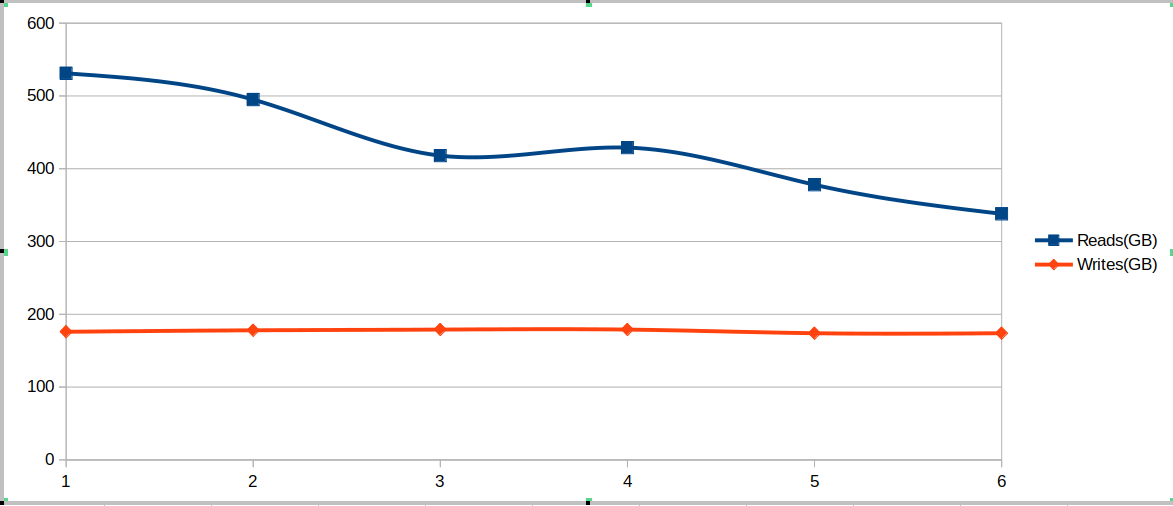
\includegraphics[width=12cm,height=6cm]{./fig/rw_pr_pc_th.png}
    \caption{Read-Write traffic over time for PageCache Page Rank
    TeraHeap Spark investigation.}
    \label{fig:rw_pr_pc_th}
\end{figure*}


\subsection{Is Spark in need of Java Heap or more cache for I/O?}

Spark's memory management is critical for the performance of big data
analytics applications. In Spark, memory is divided into three
regions: heap memory, execution memory, and storage memory. The heap
memory is used for JVM objects and the Spark driver. Execution memory
is used for storing data during shuffle and join operations and for
caching frequently accessed data. Storage memory is used for storing
data that is too large to fit in the execution memory. Spark's memory
management system automatically manages the memory allocation and
deallocation process based on the workload and available resources.
This dynamic allocation helps to avoid memory fragmentation and
optimize resource utilization. Additionally, Spark uses a combination
of in-memory and disk-based storage to provide efficient data access.
Spark provides various storage levels, including MEMORY-ONLY,
MEMORY-AND-DISK, and DISK-ONLY, to allow users to balance between
memory usage and data availability. We choose MEMORY-AND-DISK to cache
50\% of the RDDs in memory and 50\%s off-heap, in the storage device,
to balance memory and storage usage. Spark needs significant amounts
of memory even with the use of an off-heap compute cache. Using
off-heap mechanisms denotes I/O and I/O is in need of an I/O cache
i.e. the Linux PageCache. Since our spark applications run within a
memory-limited cgroup in order to assure fair performance in-between
instances, that means that we have to investigate how the different
Spark workloads that we are going to use for our evaluation are going
to perform with different amounts of H1 (Java Heap) and I/O cache.
Increasing/decreasing H1 automaticaly does the opposite to the I/O
cache so the mechanism is simple: we manually tune these parameters
and investigate how the workloads perform. At first we investigate the
performance of TeraHeap Spark regarding these two parameters. Our
machine uses 256 GB total DRAM and 16 single-NUMA island CPUs.


Figure 1 shows performance of single-instance TeraHeap Spark
running PageRank with adjustable size for H1 while PageCache is kept
steady at 16 GB. This graph shows that decreasing the size of H1
indicates a significant increase to Minor GC and a slight increase to
Major GC. Figure 2 justifies these claims by showing the obvious
decrease of the number of minor gcs. Figure 3 shows performance of
single-instance TeraHeap Spark running PageRank with adjustable size
for PageCache while H1 is kept steady at 44 GB. This graph shows that
decreasing the size of PageCache indicates no changes to other time.
Figure 4 justifies these claims by showing the obvious decrease of the
number of minor gcs.
 

Figure \ref{fig:linr_h1_native} shows performance of single-instance
Native Spark running LinearRegression with adjustable size for H1
while PageCache is kept steady at 10 GB. This graph shows that
decreasing the size of H1 indicates a significant increase to Major GC
and a slight increase to S/D. Other time remains the same. Figure
\ref{fig:gcs_linr_h1_native} and \ref{fig:rw_linr_h1_native} justify
these numbers by showing the number of minor-major gcs to decrease
while H1 increases (gc time) and the read-write traffic to remain
steady (other). Figure \ref{fig:linr_pc_th} shows performance of
single-instance TeraHeap Spark running LinearRegression with
adjustable size for PageCache while H1 is kept steady at 40 GB. This
graph shows that decreasing the size of PageCache indicates
significant changes to Other time. GC time should remain the same as
H1 remains steady. Figure \ref{fig:gcs_linr_pc_th} and
\ref{fig:rw_linr_pc_th} justify these numbers by showing the number of
minor-major gcs to remain the same while read traffic decreases as
PageCache increases. Figure \ref{fig:linr_h1_th} shows performance of
single-instance TeraHeap Spark running LinearRegression with
adjustable size for H1 while PageCache is kept steady at 10 GB. This
graph shows that decreasing the size of H1 indicates no increase to
any stat. Figure \ref{fig:gcs_linr_h1_th} and \ref{fig:rw_linr_h1_th}
justify these numbers by showing the number of major gcs to stay the
same while H1 increases (gc time) and the read-write traffic to remain
steady (other). Figure \ref{fig:linr_pc_th} shows performance of
single-instance TeraHeap Spark running LinearRegression with
adjustable size for PageCache while H1 is kept steady at 40 GB. This
graph shows that decreasing the size of PageCache indicates no changes
to Other time. So changes to PageCache do not affect this workload.
Figure \ref{fig:gcs_linr_pc_th} and \ref{fig:rw_linr_pc_th} justify
these numbers by showing the number of minor-major gcs as well as
read-write traffic to remain the same.

\subsection{What kind of metrics should someone use to be
accurate when measuring performance?} When measuring performance, it's
important to choose metrics that provide a comprehensive view of the
system's behavior. In the case of measuring the performance of Spark
instances, there are several key metrics that one should consider.
These include heap capacity, which is the amount of memory allocated
to the Java Virtual Machine (JVM) running Spark, and total memory used
by the instance, which is the actual amount of memory consumed by the
Spark instance, as measured by the cgroup budget. GC time is also an
important metric, as it measures the amount of time spent by the JVM
garbage collector in freeing up memory. Serialization/deserialization
time, measured using a Java async profiler, is important for
understanding how much time is spent in this operation, which can be a
bottleneck for some workloads. Other time, which is simply the
difference between total time and GC and serialization/deserialization
time, can provide insight into other factors that may be affecting
performance, but mainly includes the time spent in I/O and also the
time spent by mutator threads to run the application code. Device
traffic, measured using iostat, is important for understanding how
much data is being read from and written to storage devices. CPU idle
and IO wait, measured using mpstat, can help identify how much of the
CPU and I/O resources are being utilized. Finally, average throughput,
measured using Spark Bench, is a good indicator of the overall
performance of the system. Other metrics, such as the total amount of
data processed and the number of minor and major garbage collections,
as measured using jstat, can also provide valuable insights into
system behavior. By considering a range of metrics, one can get a more
accurate and comprehensive view of the performance of Spark instances.

\subsection{Why would someone choose to run the workloads
concurrently and not one by one?} The concurrent
execution of multiple workloads on a single server has emerged
as a strategy to improve efficiency and productivity. This section
aims to explore the reasons why running multiple workloads
concurrently offers significant advantages over sequential execution.

Concurrent execution of workloads provides several benefits.
Firstly, it enables optimal resource utilization by effectively
leveraging the available hardware resources, including CPUs, memory,
and storage. Rather than leaving server resources idle between
workloads, concurrent execution ensures their efficient utilization,
leading to improved throughput and enhanced server efficiency.
Additionally, the consolidation of multiple workloads onto a single
server reduces hardware footprint, simplifies management, and
minimizes operational costs associated with managing multiple servers.

Another advantage is the potential for increased throughput. By
executing multiple workloads concurrently, tasks progress
simultaneously, resulting in faster completion and higher overall
throughput. This approach is particularly valuable when workloads
exhibit varying levels of computational intensity or have different
resource requirements. Concurrent execution allows for efficient
resource allocation, enabling each workload to access the necessary
resources and perform optimally.

Concurrent execution also facilitates workload prioritization,
allowing organizations to allocate resources based on workload
importance or urgency. By running multiple workloads concurrently,
critical or high-priority tasks can be assigned the required resources
and processed in a timely manner. This flexibility in resource
allocation and workload prioritization ensures efficient utilization
of available resources and improves overall performance.

Furthermore, the concurrent execution of workloads supports
experimentation and testing. By running workloads concurrently on the
same server, comparisons, performance benchmarking, and optimization
can be performed in a controlled environment. This concurrent
execution environment enables organizations to evaluate and fine-tune
applications effectively.

Moreover, concurrent execution of workloads allows users to run
workloads along with other users simultaneously. While this is a
method that wouldn't be considered correct in order to evaluate
something because of the interference of other applications running
concurrently, it is something common for the cloud and datacenters
where companies-users share the cloud-server.

Scalability is another advantage of concurrent execution. As data
volumes and processing demands increase, running multiple workloads
concurrently allows for horizontal scalability. Additional 
worker nodes can be added to accommodate larger workloads or handle
additional workloads without the need for significant infrastructure
changes. This scalability ensures that the system can handle growing
demands while maintaining high performance.

In conclusion, the concurrent execution of multiple workloads on
a single server offers significant advantages for performance
optimization. It enables optimal resource utilization, workload
consolidation, improved throughput, workload prioritization,
experimentation, and scalability. By carefully managing resources,
workload scheduling, and monitoring, organizations can achieve higher
performance, reduce infrastructure costs, and simplify management.

\subsection{Is cost a contributing factor to pursuing higher
throughput for a server?}
Renting servers is a common practice for organizations requiring
computational resources, and the question arises as to whether
reducing the monetary cost is possible by achieving higher throughput
and faster workload completion. The relationship between cost
reduction and achieving higher throughput on rented servers is indeed
significant. By optimizing server performance, efficiently utilizing
resources, implementing workload scheduling, and improving
productivity, organizations can realize cost savings. Achieving higher
throughput and faster workload completion can lead to a reduced rental
duration, minimizing the time and associated costs of server usage.
Efficient resource utilization and workload scheduling contribute to
cost reduction by minimizing the number of servers required and
maximizing their utilization. Rental pricing models that take into
account resource utilization or data processed can further reduce
costs for organizations achieving higher throughput. Additionally,
improved productivity resulting from higher throughput and faster
workload completion enhances overall efficiency, allowing
organizations to accomplish more work within the same rental period
and reducing rental expenses. Therefore, pursuing higher throughput
and faster workload completion offers tangible benefits in terms of
monetary cost reduction for organizations renting servers. 
\par In order to estimate the cost of our evaluation in real-world public clusters we
chose a variety of providers like Amazon, Google and Microsoft. This
way we covered the most known providers and platforms someone would
choose to run their workloads on. We chose 2 machines from each
platform identical to the specifications of our 64 and 256 GB DRAM
machines. These are the cheapest machines of that particular category
offered by the platform. We then used the platform's pricing
calculator to estimate the cost of renting that machine for the time
needed for each configuration to finish execution of all instances. Finally, we noticed that the price for
renting the storage device is really amenable to the cost for renting the machine.
